\section{Backend}

\subsection{Descrizione generale}
Con l'approfondimento del capitolato e il confronto con il proponente, il gruppo ha ritenuto di sviluppare la piattaforma individuando i principali domini su cui lavorare e procedendo nello sviluppo di questi \textbf{microservizi}. \\
I microservizi da noi individuati sono:
\begin{itemize}
	\item \textbf{Products-categories service;}
	\item \textbf{Payments-orders service;}
	\item \textbf{Carts service;}
	\item \textbf{Addresses service;}
	\item \textbf{Users service.}
\end{itemize}
Lo sviluppo di singoli servizi permette una maggiore possibilità di sviluppo in parallelo dei singoli domini grazie alla loro struttura e all'agilità degli aggiornamenti e la possibilità di gestire i dati in modo decentralizzato, allo stesso tempo è comunque necessario prestare attenzione alla comunicazione che avviene tra i vari microservizi.

\subsection{Struttura dei microservizi}
\begin{figure}[H]
	\centering
	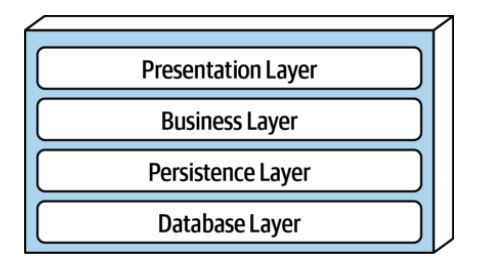
\includegraphics[scale=0.4]{Immagini/Backend/layer.png}
	\caption{layered architecture}
	\label{fig:layer}
\end{figure}
La struttura di ogni singolo servizio si basa su una Layered Architecture dove i componenti sono organizzati in vari strati che comunicano tra loro, il principale vantaggio è che risulta molto più semplice procedere ai test attraverso mock. \\
Andando ad analizzare il singolo microservizio abbiamo:
\begin{center}
	\begin{minipage}{0.3\textwidth}
		\centering
		
\includegraphics[scale=0.78]{Immagini/Backend/Amazon-DynamoDB.png}
		\captionof{figure}{DynamoDB}
	\end{minipage}
	\begin{minipage}{0.3\textwidth}
		\centering
		
\includegraphics[scale=0.19]{Immagini/Backend/AWSLambda.png}
		\captionof{figure}{Lambda}
	\end{minipage}
	\begin{minipage}{0.3\textwidth}
		\centering
		
\includegraphics[scale=0.26]{Immagini/Backend/Gateway.png}
		\captionof{figure}{API Gateway}
	\end{minipage}
\end{center}
\begin{itemize}
	\item \textbf{DynamoDB:} per gestire i vari dati;
	\item \textbf{Lambda:} le funzioni che lavorano sui dati del database;
	\item \textbf{API Gateway:} riceve e gestisce le richieste del client richiamando le lambda e restituendone i risultati.
\end{itemize}

\subsubsection{Products-categories service}
\begin{figure}[H]
	\centering
	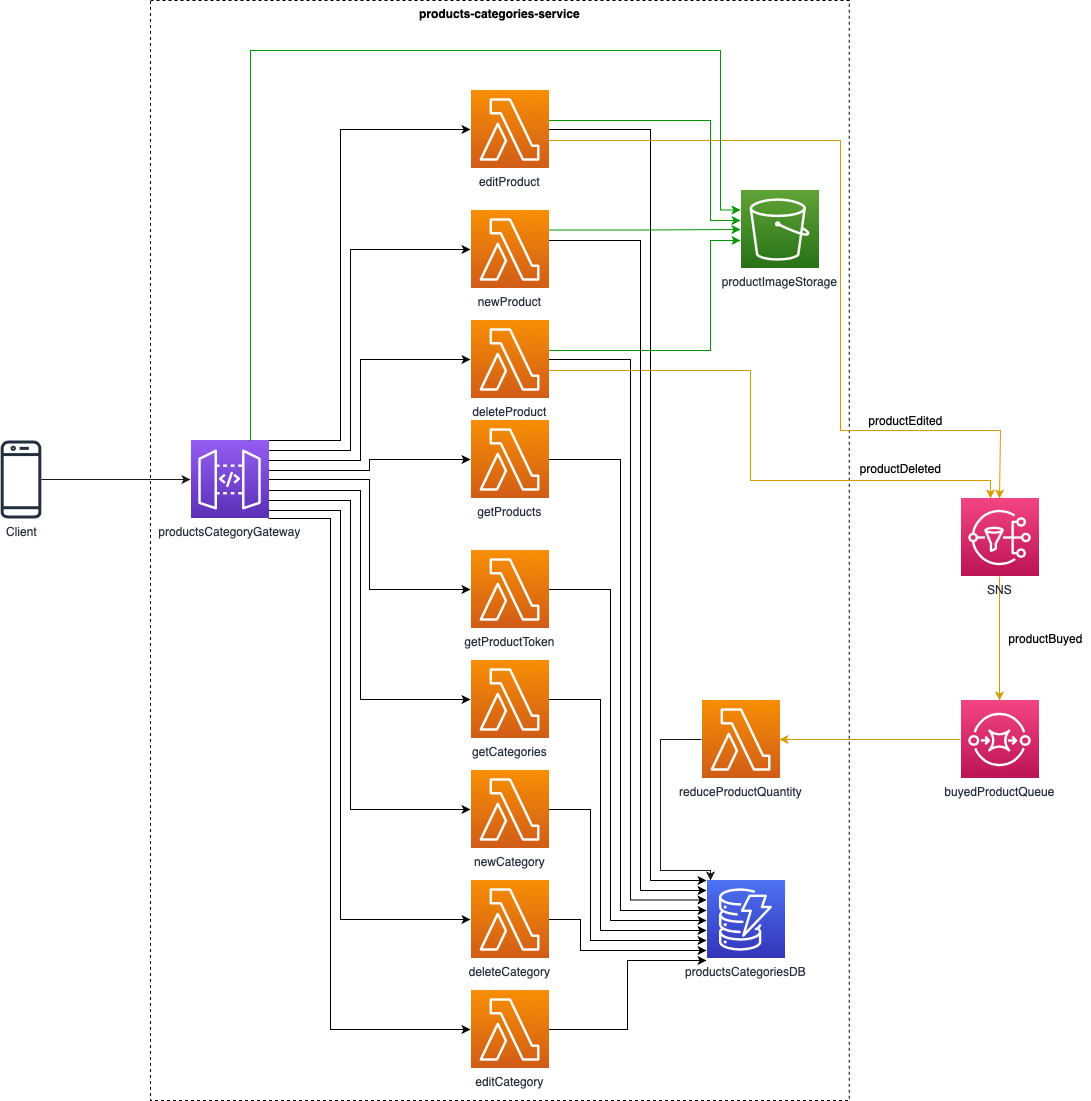
\includegraphics[scale=0.4]{Immagini/Backend/AWSProductsCategories.png}
	\caption{Products-categories service}
	\label{fig:ProductCategories}
\end{figure}

\subsubsection{Payments-orders service}
\begin{figure}[H]
	\centering
	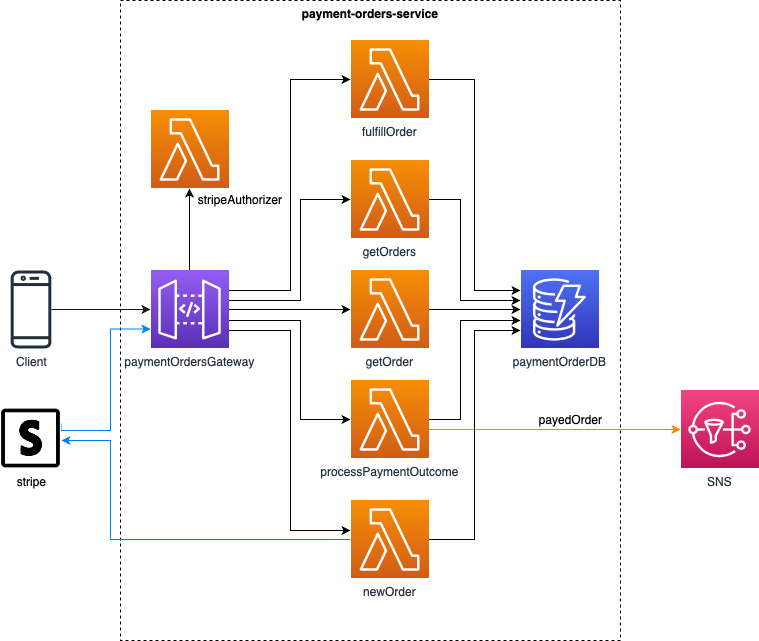
\includegraphics[scale=0.4]{Immagini/Backend/AWSPaymentOrders.png}
	\caption{Payments-orders service}
	\label{fig:Payment-orders}
\end{figure}

\subsubsection{Carts service}
\begin{figure}[H]
	\centering
	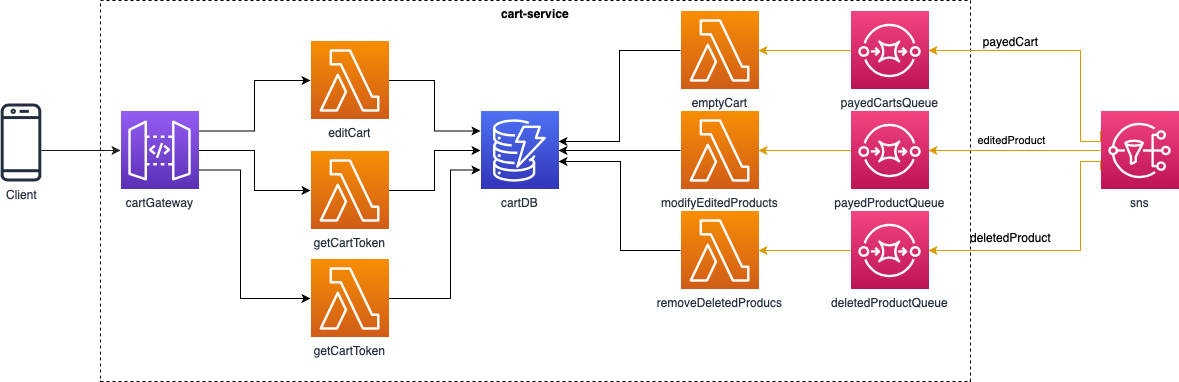
\includegraphics[scale=0.4]{Immagini/Backend/AWSCart.png}
	\caption{Carts service}
	\label{fig:Cart}
\end{figure}

\subsubsection{Addresses service}
\begin{figure}[H]
	\centering
	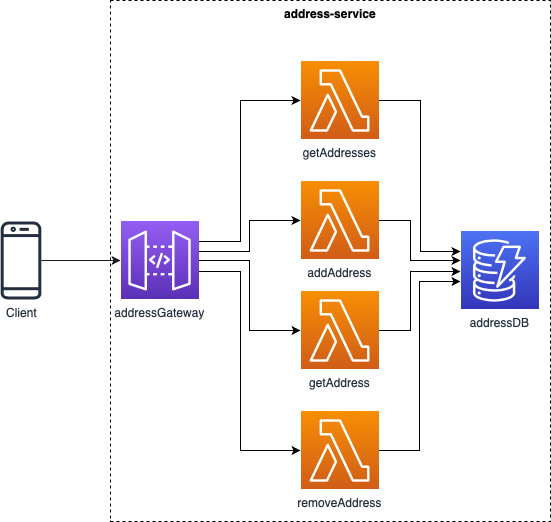
\includegraphics[scale=0.4]{Immagini/Backend/AWSAddresses.png}
	\caption{Addresses service}
	\label{fig:Adresses}
\end{figure}
\subsubsection{Users service}
\begin{figure}[H]
	\centering
	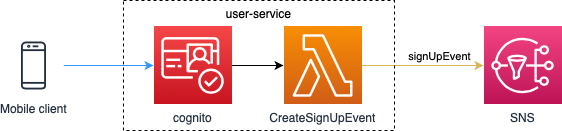
\includegraphics[scale=0.7]{Immagini/Backend/AWSUserService.png}
	\caption{Users service}
	\label{fig:Users}
\end{figure}
\subsection{Struttura del backend}
\begin{figure}[H]
	\centering
	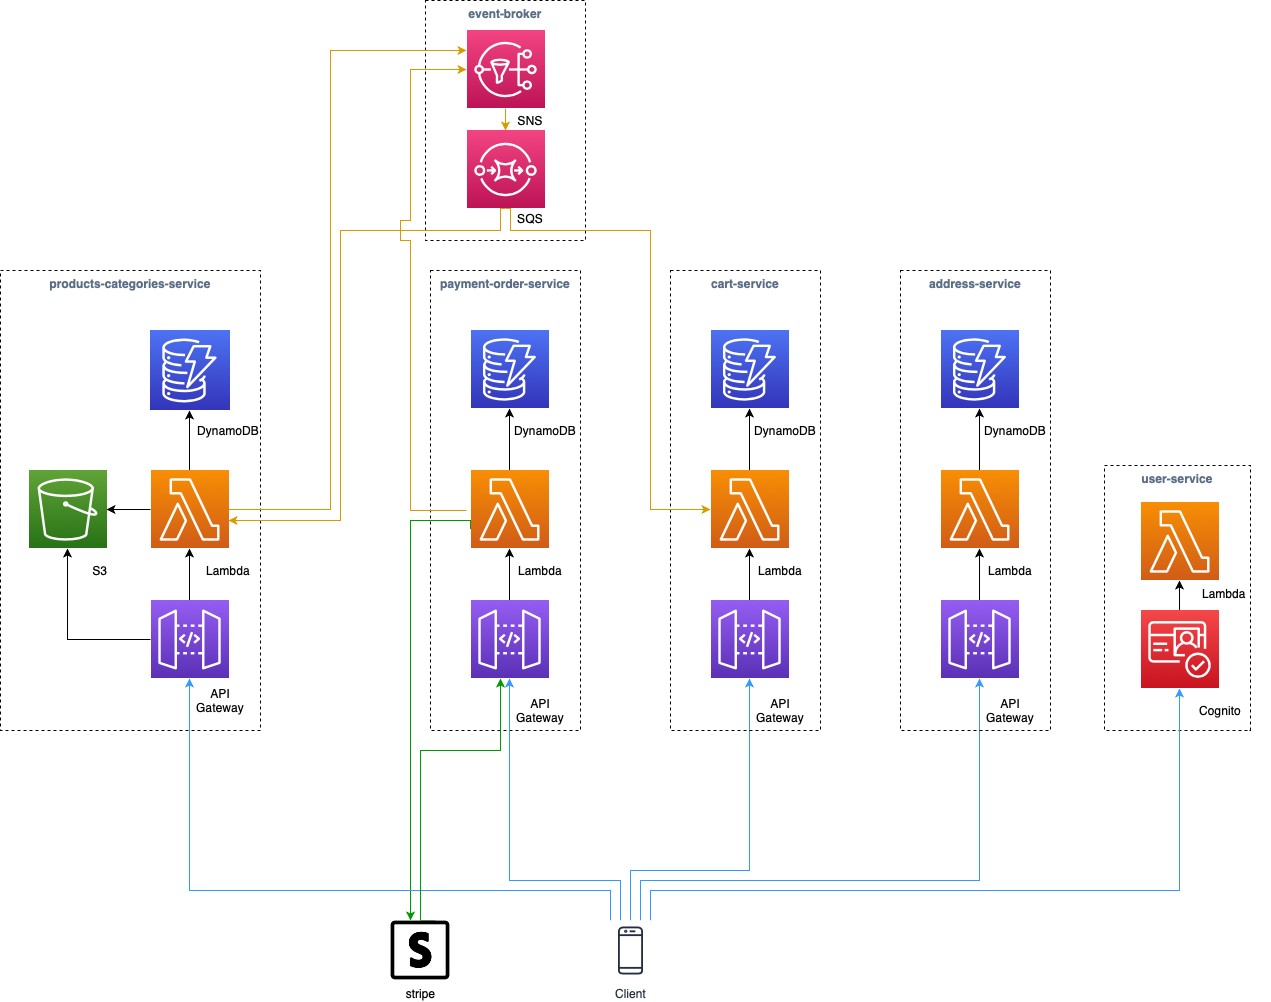
\includegraphics[scale=0.4]{Immagini/Backend/AWSArchitecture.png}
	\caption{Architettura backend}
	\label{fig:backend}
\end{figure}
Per slegare i microservizi tra di loro abbiamo usato 2 strategie. La prima consiste nel gestire le chiamate asincrone attraverso SNS il servizio che fa da event broker su AWS, eliminando così lo sviluppo di integrazioni tra micro servizi e limitandosi a quelle per il message broker.
La seconda invece è pensata per eliminare le chiamate sincrone tra micro servizi, come quelle di validazione. Per far ciò utilizziamo la firma digitale legata a un micro servizio per verificare l'integrità delle richieste del client, sostituendo così le varie integrazioni necessarie a un semplice check attraverso la chiave pubblica del micro servizio.

\subsection{Diagrammi di sequenza}
Di seguito sono riportati due diagrammi di sequenza per due principali operazioni:
\begin{itemize}
	\item l'acquisto di un carrello;
	\item la ricezione di un evento tramite Stripe Hooks.
\end{itemize}
\begin{figure}[H]
	\centering
	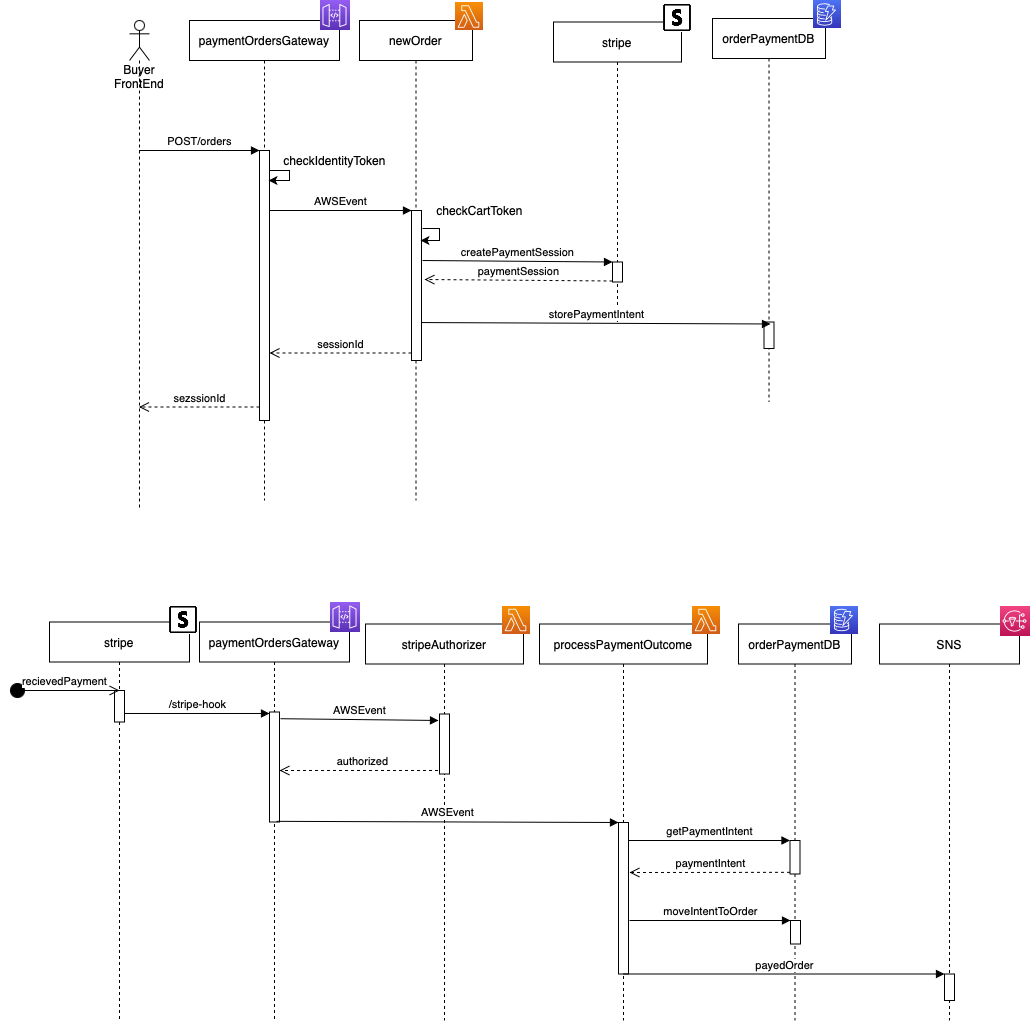
\includegraphics[scale=0.5]{Immagini/Backend/Diagrammiseq.png}
	\caption{Diagrammi di sequenza}
	\label{fig:Diagrammiseq}
\end{figure}